\documentclass[11pt,oneside]{report}

%%% Load some useful packages:
%% "New" LaTeX2e graphics support.
\usepackage{graphicx}
%%	using final option to force graphics to be included even in draft mode
%\usepackage[final]{graphicx}
%% Tell graphicx the default directory for all figures
\graphicspath{{figures/}}

%% Enable subfigure support
\usepackage{subfigure}

%% Make subsubsections numbered and included in ToC
\setcounter{secnumdepth}{3}
\setcounter{tocdepth}{3}

%% Package to linebreak URLs in a sane manner.
\usepackage{url}

%% Define a new 'smallurl' style for the package that will use a smaller font.
\makeatletter
\def\url@smallurlstyle{%
  \@ifundefined{selectfont}{\def\UrlFont{\sf}}{\def\UrlFont{\small\ttfamily}}}
\makeatother
%% Now actually use the newly defined style.
\urlstyle{smallurl}

%% Define 'tinyurl' style for even smaller URLs (such as in tables)
\makeatletter
\def\url@tinyurlstyle{%
  \@ifundefined{selectfont}{\def\UrlFont{\sf}}{\def\UrlFont{\scriptsize\ttfamily}}}
\makeatother

%% Provides additional functionality for tabular environments
\usepackage{array}

%% Puts space after macros, unless followed by punctuation
\usepackage{xspace}

%% Make margins less ridiculous
\usepackage{fullpage}

%% Allows insertion of fixme notes for future work
\usepackage[footnote, nomargin]{fixme}

%%%% Turned off for tech report, should be turned on for research portfolio
%% Turn on double spacing
%\usepackage{setspace}
%\doublespacing

%% Make URLs clickable
%\usepackage[colorlinks, bookmarks=false]{hyperref}
\usepackage[colorlinks, bookmarks=true]{hyperref}

%% Since I'm using the LaTeX Makefile that uses dvips, I need this
%% package to make URLs break nicely
\usepackage{breakurl}

\usepackage{amsmath,amsfonts}
\numberwithin{equation}{subsection}
%%\usepackage{nonfloat}
\usepackage{bbm}
\usepackage{setspace}
\onehalfspacing
\usepackage{tabularx}

%%% End of preamble
\begin{document}

\title{Literature Review on Time Series Indexing}
\author{Pavel V. Senin \\
Collaborative Software Development Lab \\
Department of Information and Computer Sciences \\
University of Hawaii \\
Honolulu, HI \\
senin@hawaii.edu \\
\\
CSDL Technical Report 09-08 \\
\url{http://csdl.ics.hawaii.edu/techreports/09-08/09-08.pdf}
}
\date{April 2009\\[3pt]
Copyright \copyright\ Pavel V. Senin 2009}

%%% Create the title page from all the information above. Note that the
%%% titlepage is outside the front matter.
\maketitle

%% Philip suggests it needs a ToC
\tableofcontents

\begin{abstract}
Similarity search in time-series databases become an active research area in the past decade corresponding to the tremendous growth of the amount of temporal data collected and publicly available. The complexity of this similarity problem lies in the high dimensionality of the temporal data making convenient methods to fail. The most promising aproaches involve dimensionality reduction and indexing techniques wich are the subject of this review. While starting with general introduction into the time-series and classical time-series analyses we will discuss in details time-series normalization techniques and relevant distance metrics following with the review of the dimensionality-reduction and indexing methods proposed up to date.
\end{abstract}

%% Start with introduction
\chapter{Introduction}\label{chapter_introduction}
\textit{The central issue I address in the dissertation is a possibility of recurrent behaviors discovery from 
publicly available software process artifacts by leveraging data mining and knowledge discovery techniques. 
In particular I explored an approach of discovering of recurrent behaviors through the mining of time series that
are constructed by temporal ordering of measurements extracted from software process artifacts.
Further, I shall propose a novel technique for characteristic patterns discovery from time series and show its 
applicability to the problem at hands.}

\textit{The problem's background is provided in the Section \ref{section_background}. 
Section \ref{section_software_process_design} presents classical approaches for software process design and shows its limitations.
Section \ref{section_research_hypothesis} introduces the research hypothesis.
Section \ref{knowledge_discovery} provides a background into the problem of knowledge discovery 
from time-series.
Section \ref{section_trajectory_definition} connects two problems and provides definitions.
Section \ref{section_contributions} enumerates main contributions of the thesis, 
while section \ref{section_organization} explains the thesis organization.}

%
% >> section
%
\section{Background}\label{section_background}
Contemporary software projects concern with development of complex software systems and typically have 
a considerably long life-cycle - well over decade.
A project's development and maintenance activities are usually carried out by geographically 
distributed teams and individuals. The development pace, the experience, and the structure of the 
development team continuously change with project progression and as developers joining and leaving. 
When combined with schedule and requirements adjustments, these create numerous difficulties 
for developers, users, and stakeholders, ultimately affecting the project success \cite{citeulike:2207657}. 

This software development complexity phenomena was identified in 1968 as ``Software crisis'' 
\cite{naur_crisis_68}, and was addressed by bringing the research and the practice of software development 
(or as it was called ``programming'') under the umbrella of Engineering - in an effort to provide 
the control over the process of software development. 
Following the engineering paradigm, numerous methodologies and models of software design and development 
process, known as \textit{software processes}, were proposed \cite{citeulike:10002165}.

\begin{defn}\label{def_process}
A \textbf{\textit{Software Process}} defines a sequence of activities performed in order 
to design, develop, and maintain software systems.
\end{defn}
Examples of such activities include requirements collection and creation of UML diagrams, 
requirements testing, code development,  testing, etc. The intent behind a software process is 
to provide a control over software evolution by implementing a global strategy and by structuring
and coordinating human activities in order to achieve the goal - deliver a functional software system 
on time and under the budget. 

Since then, much research has been done on software processes resulting in a number
of software development models and paradigms. Some of these were widely accepted by practitioners 
and evolved into industrial standards for software development processes such as CMM, ISO, PSP, 
and others \cite{citeulike:5043104}. However, in spite of this effort, industrial software 
development remains error-prone and more than half of all 
commercial software development projects ending up failing or being very poorly executed 
(Rubinstein, ``Chaos Reports'', 2006) \cite{chaos2006}. Some of them are abandoned due to running 
over budget, some are delivered with such low quality, or so late, that they are useless, and some, 
when delivered, are never used because they do not fulfill requirements. 

Through the analyses of software project failures, it was acknowledged, that the engineering 
paradigm might not be the best way to provide a control over software development processes 
(\cite{citeulike:3729379} \cite{citeulike:5203446}) due to the fact that Software engineering 
is dealing with significantly different from other Engineering fields problems \cite{citeulike:2207657} .
The chief argument supporting this point of view is the drastic difference in the cost model:
while in Software Engineering there is almost no cost associated with materials and 
fabrication, these usually dominate cost in all other Engineering disciplines, but, 
ironically, Software Engineering is suffering from the costs and challenges associated with 
continuous re-design of the product and its design processes - the issue which is 
hardly seen at all in other Engineering areas. 
Further, it was found, that most of the engineering-like models are rigid, ``context-free'',
and rather prescriptive, i.e. they are universally defined independently of a particular 
organizational structure or a project specificities \cite{sacchi_2001}, and while they 
structure processes and provide the control, following them does not guarantee the success.
Yet another argument supporting alternative to engineering approaches is the increasing 
understanding and appreciation of a human role in software development processes over tools, 
technologies, and standards \cite{citeulike:6580825} \cite{citeulike:149387}
\cite{1605185} \cite{citeulike:113403} \cite{1605188} \cite{citeulike:12743107}. 

Along with Software Engineering, a number of alternative, flexible and user-oriented software processes 
emerged from academy, hobbyists, and practitioners addressing aforementioned issues \cite{citeulike:3729379}. 
Among others, the Free/Libre/Open-Source Software model (FLOSS) and the software craftsmanship  
approaches gained a significant credibility in community. 
While the former \textit{holistic} software process paradigm emphasizes loosely-organized 
collaboration, frequent releases, and effectively removes the boundary between developers 
and customers, the latter, human-centric approach, is built upon the roles of highly 
motivated skilled individuals \cite{citeulike:262020} \cite{citeulike:2759198}. 

Nevertheless, alternative processes were found to be plagued by the same complexity issues. 
As it was shown, most of FLOSS projects never reach a ``magic'' 1.0 version \cite{citeulike:12480029}. 
Among others, the great "infant mortality rate" of FLOSS projects was related to a burnout, 
inability to acquire a critical mass of users, loss of leading developer(s), and forking \cite{richter2007critique}. 
Software craftsmanship, from other hands, not only challenges developers with technological advances 
requiring continuous skills improvement, but creates significant cost and effort estimation difficulties for
stakeholders and project managers \cite{citeulike:11058784}. However, despite to these issues, 
the alternative processes proved that the disciplined manner of programming and the modularization  
of the software are capable of delivering large and reliable software systems, most notable Linux OS,
suggesting that community-driven processes as good as industrial engineering-like processes.

Currently, it is widely acknowledged, that there exists no single ``silver bullet'' process which 
can bring a software development project to success \cite{citeulike:1986013}. 
Processes are numerous, each has advantages and drawbacks, and each is accompanied with 
numerous application recommendations, success stories, and with failure experiences. Nevertheless,
the alarming rate of failing projects suggests that our understanding of software process ``mechanics''  
is limited and insufficient\cite{citeulike:12550665}. 
The enormous cost of the lost effort, measured in hundreds of billions of US dollars 
\cite{citeulike:2207657} \cite{citeulike:2207653} \cite{citeulike:2207655}, 
continues to provide motivation for further research on software processes. 

%
% >> section
%
\section{Software process design}\label{section_software_process_design}
Traditionally, approaches to software process design and improvement are divided into two distinct categories. 

The first category of software process design approaches consists of traditional to engineering 
\textit{top-down} prescriptive techniques through 
\textit{proposing a process based on specific patterns of software development}. 
For example, the Waterfall Model process proposes a sequential pattern in which developers first create a 
Requirements document, then create a Design, then create an Implementation, and finally develop Tests. 
The Test Driven Development process, from other hands, proposes an iterative behavioral pattern in which
the developer must first write a test case, then write the code to implement that test case, then re-factor the 
system for maximum clarity and minimal code duplication \cite{citeulike:6086365}. 

While the top-down approach follows the usual path of trials and errors, and seems to be an extension 
of natural to humans creative processes of invention and experimentation, 
the ``invention'' of an adequate to the task software process is far from trivial 
\cite{citeulike:5043104} \cite{citeulike:1986013}. Moreover, an evaluation cycle of an invented process
is usually very expensive and considerably long.
In addition, it was shown that the process inventors are often limited in their scope and tend to assume 
idealized versions of real processes, thus, often produce ``paper lions'' - process models which are 
likely to be disruptive and unacceptable for end users, at least in their proposed form 
\cite{citeulike:9758924}, which creates a large discrepancy between actions that supposed to be done for 
the novel process and what was actually performed by particular individual or the team.

The second category of software design approaches consists of \textit{bottom-up} techniques 
that focus on a \textit{performed process reconstruction through noticing of recurrent development 
events and behaviors} or as it also called \textit{process enactment}. 
Usually, the process reconstruction task is viewed as a two-levels problem where the first level 
consists of a patterns discovery (segmentation) while the second level consists of patterns recognition 
and their network analysis \cite{citeulike:2703162}.
One of the first works in this category was by Cook and Wolf, where they show a
possibility of automated extraction of a process model through the mining of recorded 
process event logs \cite{citeulike:328044} \cite{citeulike:5120757} \cite{citeulike:5128143}. 
Later work by Huo et al. shows that it is also possible to improve an existing process
through the event logs analysis \cite{citeulike:7691059} \cite{citeulike:7690766}. 

While the bottom-up approaches seem to be more systematic and potentially less complex than invention, 
they also affected by a number of issues. A chief among these is the observability issue - 
it is usually very difficult to conduct a full depth study on a live project due to the privacy concerns. 
Moreover, it is expensive to observe a process performed by a team for a whole life-cycle of a project. 
Yet another issue is the capacity of currently available process discovery techniques - 
typically these need to be supervised by experts and finely tuned in order to reconstruct 
distributed and concurrent processes. 

Nevertheless, despite to their differences, both techniques for software process design are 
producing process models that effectively are the series of actions that must be performed successively 
(sequentially and sometimes iteratively) in order to deliver a software. 
In order to produce the viable model, the ``process inventors'' put the best of their knowledge, experience,
creativity, and logical reasoning into the proposed sequence of steps, while ``process re-constructors 
strive to eliminate the noise and to converge to a concise process model that is supported by the 
majority of observations. 
This attention to synthesis of sequential steps, leaves other phenomenas, such as team's structure, work schedule, 
developer's discipline, their behaviors, and motivation behind. While this issue was recognized previously
and resulted in a number of studies which called for attention of human element in software production 
\cite{citeulike:149387} \cite{citeulike:113403} \cite{citeulike:205322} \cite{citeulike:12798652}, 
it is still largely ignored in industrial practices \cite{citeulike:12798659}, mostly due to the 
difficulties in benefit estimation \cite{citeulike:12798662} \cite{csdl2-12-11}.

%
% >> section
%
\section{Free/Libre Open Source processes}\label{floss_processes}
Along with growing amount of publicly available software, it became obvious, that self-organizing communities of 
mostly ``recreational'' software developers and active users are capable to successfully manage large code base, 
but to deliver software increasingly complex and surprisingly popular.
Many of large, ``global'' open source software development projects, such as Linux and its derivatives, 
Gnome, Apache HTTP Server, MySQL, and others, not only have comparable with industrial projects development team 
and code-base sizes, but the same average defect rate \cite{coverity2012}. 
These facts have attracted a considerable attention from industry and many organizations 
seek to emulate successful open source software processes in traditional ``closed source'' environment 
\cite{oss_virtual_organizations} \cite{oss_balance} \cite{oss_hp} \cite{oss_4industry}. 

\begin{figure}[ht!]
   \centering
   \includegraphics[width=140mm]{figures/Linus.Kernel.ps}
   \caption{A Torvald's response suggesting that practical reasons, the ``real-life'', should be always considered 
   over specifications.
   Excerpt from the Linux mailing list. \url{http://lkml.indiana.edu/hypermail/linux/kernel/0509.3/1441.html}}
   \label{fig:kernel}
\end{figure}

If we consider this as an assertion that open-source software processes are at least as good as engineering-like 
software process models, then, the freely available open-source process software artifacts potentially bear an 
incredible wealth of the information worth of studying. Moreover, the striking differences of open-source processes 
from a traditional software development could potentially reveal novel software processes and their aspects that 
were previously not accounted for. 
For example, consider that the most significant document in industrial software processes - a specification - 
is rarely considered at all in open source world. In FLOSS projects the software look and its functionality are 
rather viewed as open-end questions. Even in the Linux kernel development, which is probably one of the few strictly 
moderated FLOSS development processes, developers prise practical reasons over specifications 
\ref{fig:kernel}.

Yet another source of motivation for studying of public FLOSS software process artifacts comes from the fact that 
in order to facilitate the distributed FLOSS software development processes, the community is highly encouraging
developers to commit their changes rather often \cite{so-checkin} \cite{git-best-practices1}.
The frequent commits and the changes visibility practice is often cited as vital for health of software 
process as mentioned in some lengthy discussions: ``\textit{Don't Go Dark}'' \cite{checkin-dgd-2008}, 
``\textit{Check In Early, Check In Often}'' \cite{checkin-ch-2012}. Potentially, frequent commits create artifacts 
trails that provide finer resolution into project development and allow more thorough process recovery.

%
% >> section
%
\section{Public software repositories}\label{section_public_repositories}
Recently, the aforementioned situation changed, and the interest for process enactment and reconstruction, 
as well as attention to the human-specific components of software processes has been revived. 
This change is driven by the increase in public data that are made available by the proliferation of open 
source communities.

Currently, with accessible personal computers, friendly software development toolkits, and due to massification
of the use of the web as
a platform for collaborative work, small-scale commercial and recreational 
programming become very popular. 
Today, free code hosting sites such as SourceForge, GoggleCode, and GitHub host thousands of 
Free/Libre Open Source Software (FLOSS) projects.
These publicly offer numerous software artifacts such as design documents, source codes, bugs and issue records, and 
developers and users communications.
Further, Q\&A and social websites for developers such as StackOverflow, Biostars, TopCoder and others becoming 
increasingly popular among the software developers as places for exchanging experiences, learning new tricks, and 
improving skills, plus, they offer anonymized data back to the community.

The public availability of numerous software process artifacts effectively removes not only the high cost of observation, 
but most of the privacy concerns - the two issues that previously made any large-scale analysis of software projects 
unfeasible for most researchers.

Scientific community response on the availability of public artifacts was overwhelming, and a number of 
venues was established addressing the increased interest. 
Since 2004, the International Conference on Software Engineering (ICSE) hosts a Working Conference on 
Mining Software Repositories (MSR). The original call for papers stated MSR's purpose as 
\textit{``... to use the data stored in these software repositories to further understanding of software 
development practices ... [and enable repositories to be] used by researchers to gain empirically based 
understanding of software development, and by software practitioners to predict and plan various aspects 
of their project''} \cite{msr2004} \cite{citeulike:7853299}. 
Several other venues: International Conference on Predictive Models in Software Engineering \cite{promise12}, 
International Conference on Open Source Systems, the Workshop on Public Data about Software Development, 
and the International Workshop on Emerging Trends in FLOSS Research have also played
an important role in shaping and advancing this research domain.

Some of the published work addresses the software process discovery. Among others, most notable and 
relevant to my research is work by Jensen \& Scacchi. In their early work, they demonstrated, that 
information reflecting software processes can be gathered from public systems \cite{citeulike:12550640}. 
Later, in \cite{citeulike:5043664} and \cite{citeulike:5128808}, they show, that by manual mapping of 
collected process evidence to a pre-defined process meta-model it is possible to reconstruct some 
of the FLOSS processes. 
Another closely related to my research is work by Hindle et al. where they has shown that it is possible to 
discover software process evidence through partitioning \cite{citeulike:10377366}.

However, the research work based on mining of software process artifacts shows, that while public availability 
of artifacts is minimizing observability and privacy issues, the nature of these artifacts creates a number of 
challenges which I discuss in the chapter X, which limit the possible scope of the research and significantly 
elevate the complexity of the process discovery effectively rendering previously designed techniques inefficient.
Thus, the novel analysis and discovery techniques are needed to be developed for public software process artifacts 
analysis \cite{citeulike:7853299}.
% when ``\textit{... going beyond code and bugs...}'' 

%
% >> section
%
\section{Research hypothesis, scope of the dissertation}\label{section_research_hypothesis}
In previous sections, I have outlined the evidence of a limited performance of existing engineering-like 
software processes (Section \ref{section_background}),
as well the oversight of a variety of human factors that fall beyond a typical sequence of development 
actions by traditional approaches to software process design (Section \ref{section_software_process_design}).
Then, I have identified a few differences of FLOSS processes from traditional Software Engineering 
(Section \ref{floss_processes}), which can potentially shed light on human-driven aspects of software development.
Finally, I have pointed out a growing wealth of publicly available software process artifacts 
(Section \ref{section_public_repositories}) that is worth to explore for a better understanding not only 
FLOSS software processes, but their human factors. All this provided a motivation to my exploratory study, 
whose details I outline in this section.

In my work, I attempted to explore the possibility of discovery of a specific human-driven aspect in 
FLOSS software development that is a \textit{\textbf{behavior}}, which I define as the mannerism in which a 
developer, or a team, conduct their everyday work. 
In particular, I explore the possibility of discovery of \textit{recurrent behaviors}, i.e. behaviors supported 
by a numerous evidence, from software process artifacts. 

For example, if within an observation interval one developer frequently runs unit tests before committing 
changes into repository, while another usually commit changes without running the tests, the first developer's
habit of testing a code before the commit is a recurrent behavior that may reflect the developer's discipline,
or an unusual attention to some particular part of the code. 
Consider another example, if one of the developers usually commits code changes in mornings, while another 
developer late in the day, these two recurrent behaviors, might indicate a constraints that are put on the 
project, or the process, or on the developers themselves.
Obviously, latter behaviors should be possible to quantify by simple analysis of commit timestamps, while 
the former can be discovered by the analysis of co-occurring changes in the source code. 
Moreover, these and similar recurrent behaviors could be further associated with certain project's or process 
traits, such as pace, agility, size, complexity, code quality and others, which will not only extend our 
knowledge of human factors in software processes, but will lay a foundation for future research in software 
processes.

To begin with, I hypothesized, that \textbf{\textit{it is possible to discover recurrent behaviors from 
publicly available software process artifacts}}. 

Following the hypothesis, I have investigated a number of publicly available software repositories,
their artifacts, and a number of applicable data-mining techniques in a preliminary exploratory study 
\cite{csdl2-10-09}. However, similarly to other studies in the field, I have discovered, that while FLOSS 
process artifacts are numerous and readily accessible, their irregular, snapshot-like nature and the poor 
informational content significantly limit the applicability of known techniques for process mining.

In order to overcome this issue, I have casted the initial problem of event-based recurrent behaviors 
discovery into more generic problem of knowledge discovery from time series and approached it
by developing a novel technique for interpretable comparative analysis of time series that allows 
characteristic patterns discovery and ranking called SAX-VSM \cite{sax-vsm}. 

Further, I have developed a software artifacts analysis framework, called Software Trajectory Analysis, 
which aids in software artifacts collection, software process and product evolutionary metrics extraction, 
and their comparative analyses that enable discovery and ranking of characteristic patterns.


 in rank highlight is  transformation into  and by using I approached the problem of knowledge discovery 

developed a 
software process artifacts mining framework called Software Trajectory Analysis which is built upon 
a novel technique for comparative analysis of time series that allows characteristic patterns discovery 
and ranking.

This dissertation presents its results, as well as introduces a novel data mining technique designed to 
alleviate difficulties with interpretability of quantitative results obtained through mining of software
artifacts trails. 

%
% >> section
%
\section{Knowledge discovery from time series}\label{section_knowledge_discovery}
In data mining, time series are used as a proxy representing a vast variety of real-life phenomena 
in wide range of fields including, but not limited to physics, medicine, meteorology, 
music, motion capture, image recognition, signal processing, and text mining. 
While time series usually directly represent observed phenomenas by capturing their measurable evolution in time, 
the pseudo time series often used for representation of various high-dimensional data 
by combining data points into ordered sequences. 
For example in spectrography data values are ordered by component wavelengths \cite{citeulike:12550833};
in shape analysis the order is the clockwise walk direction starting from a
specific point in the outline \cite{citeulike:12550835}, in image classification the numbers of pixels
are sorted by color component values \cite{citeulike:2900542}.

Many important problems of knowledge discovery from time series reduce to the core task of finding 
characteristic, likely to be repeated, sub-sequences in a longer time series. 
In the early work these were called as 
\textit{frequent patterns} \cite{citeulike:5159615}, 
\textit{approximate periodic patterns} \cite{citeulike:1959582},
\textit{primitive shapes} \cite{citeulike:5898869}, 
\textit{class prototypes} \cite{citeulike:4406444}, 
or \textit{understandable patterns} \cite{citeulike:3978076}. 
Later, similarly to Bioinformatics, these were unified under the term \textit{motif} \cite{citeulike:3977965}.
Once found, motifs can be used for a hypothesis generation by finding their associations with known,
or unknown phenomenas \cite{citeulike:3977965}. 

The recent advances in semi-supervised and unsupervised finding of such characteristic sub-sequences, 
in particular work based on \textit{shapelets} \cite{citeulike:7344347} \cite{citeulike:11957982}
\cite{citeulike:12552293} and \textit{bag of patterns} \cite{citeulike:10525778}, show a great potential 
of application of time series data-mining techniques to a wide variety of high-dimensional data.

Unfortunately, both techniques provide a limited insight into the data and suffer from performance issues. 
While exact shapelet techniques allow discovery of class-characteristic patterns and facilitate classification,
algorithm is almost quadratic and provides limited insight into class specificities. 
The bag of patterns algorithm, while performs in a linear time, requires a previous knowledge for input parameters 
selection and does not offer class generalization.

In order to overcome this limitations, in this thesis I propose a novel approach for time-series classification and 
knowledge discovery that is called SAX-VSM and is based on symbolic approximation of time series and vector space model. 
As I shall show, SAX-VSM is capable to discover and to rank characteristic subsequences representing time series classes. 
The proposed algorithm not only facilitates classification, but provides insights into the both: classification results 
and time series classes specificities. As I shall show, by facilitating the class' characteristics patterns ranking,
SAX-VSM enables the discovery of recurrent behaviors and their heat-map like visualization. 

\section{Software trajectory analysis}\label{section_trajectory_definition}
Previously, Johnson et al. defined \textit{software metrics telemetry streams} \cite{citeulike:12550871}, 
(what they re?) and showed, that it is possible to improve software development process by using the 
knowledge extracted by experts through visual analysis of these streams.
 
Similarly to software metrics telemetry streams, I abstract software process artifact by collecting their 
metrics and arrange these measurements by artifact creation time into high-dimensional vectors. 
These non-equidistant, often sparse and uneven in length time series 
I call ``\textbf{software trajectories}''. Similarly to approximate trajectories of objects in 
a physical space, or reduced in complexity sequence of states of a dynamic system (Poincare' maps), 
the \textit{software trajectory is a curve that describes a software project progression in a space 
of a chosen metrics}.

Through an exploratory study, I have discovered, that by the comparative analysis of software trajectories 
with SAX-VSM it is possible to discover and to interpret recurrent behaviors. This workflow that 
consists of software artifacts collection, their metrics extraction, and comparative analyses I call 
\textit{\textbf{Software Trajectory Analysis}} (STA). 

In this thesis, through three case studies, I will show, that Software Trajectory Analysis is capable 
of discovering of a various characteristic patterns which ca be associated with recurrent behaviors.

\section{Contributions}\label{section_contributions}
Main contributions of my work can be summarized as follows: 
\begin{itemize}
\item I propose a novel, generic algorithm for interpretable time series classification: SAX-VSM. 
While the classification performance of this algorithm is at the level of current state of the art, 
it offers an outstanding feature - discovery, generalization, and ranking of class-characteristic features. 
This, in turn, enables knowledge discovery by offering much clearer insight into classification results than any of 
competing techniques.
In addition, SAX-VSM is very fast in classification and has a small memory footprint. 
Overall, I expect this algorithm to play an important role in future because of the growing ubiquity of time series and 
a growing interest in behaviors.
\item Powered by SAX-VSM, I design a Software Trajectory Analysis (STA) framework, and through case-studies 
show its capacity for recurrent behaviors discovery from publicly available software process
artifacts. While case studies are obviously limited, I argue that STA is a useful knowledge discovery tool applicable for a 
variety of software process artifacts and metrics. 
\item Finally, I provide SAX-VSM and STA implementations to community.
\end{itemize}

\section{Dissertation Outline}\label{section_organization}
The rest of this dissertation is organized as follows. Chapter \ref{chapter_background_work} discusses the history 
of Software Engineering, previous work in software process discovery, mining of software repositories, and current 
state of the art in time series mining. Chapter \ref{chapter_sax_vsm} proposes an algorithm for interpretable 
time series classification. Chapter \ref{chapter_sta} discusses the design of STA framework and presents case studies.
Chapter \ref{chapter_conclusions} concludes and discusses several directions for future study.

%% similarity measures
\chapter{Time-series similarity measurements.}
Previously not explored in the classical time-series analyses such as trend and seasonality identification, forecasting and others, the time-series similarity \footnote{Note that a time-series (a finite sequence of real numbers) is alternatively called ``sequence'' or ``signal'' in the literature and we might use these terms depending on the context of the reviewed paper or method.}  problem become the cornerstone problem in recently emerged data-mining applications. The ability to determine time-series similarity allows solving many general time-series KDD problems:
\begin{itemize}
	\item identifying stocks with similar movement in price \cite{citeulike:4384535} \cite{citeulike:4031865} \cite{citeulike:4025073}
	\item finding products with similar selling pattern \cite{citeulike:4326324}
	\item identifying music with the score similar to the copyrighted one \cite{citeulike:3821484} \cite{citeulike:3815076}
	\item performing speech to text conversion \cite{citeulike:3728228}
	\item verifying signatures and performing handwriting to text conversion \cite{citeulike:3733947} \cite{citeulike:3513035}
	\item finding objects with similar movement trajectories \cite{citeulike:964832} \cite{citeulike:3728229} \cite{citeulike:3815864}
	\item detecting anomalies or events in the signals \cite{citeulike:4412621} \cite{citeulike:4412617}
	\item finding developers with similar build patterns.
\end{itemize}

All of the solutions for this set of problems are based on the implementation of the time-series database enhanced by ability to process ``time-series similarity queries'' or ``range queries'' and at this point we essentially regard this problem as solved and will overlook some of the solutions in this review. 

First introduced by Goldin and Kanellakis \cite{citeulike:3815880}, the concept of the ``approximately similar time-series data'' is based on the ``user-perceived similarity'' rather than direct mathematical comparison with straightforward metrics. This very important observation essentially relaxes constraints for finding similar time-series. As an example of this relaxation, authors introduce scales and shifts in order to simulate the human ability in relating time-series features. Naming scale as the $a$ coefficient and shift as $b$ they introduced a form of the ``similarity relation'' $T_{a,b}$ with next properties:
\begin{align}
 & \text{1. } \forall \; X, \; X=T_{0,1}(X), \; \text{Reflexivity or identity transformation} \\
 & \text{2. } \text{if } X=T_{a,b}(Y) \; \text{then } Y=T_{\frac{1}{a},-\frac{b}{a}}(X) = T^{-1}_{a,b}(X), \; \text{Symmetry or inverse of $T_{a,b}$} \\
 & \text{3. } \text{if } X=T_{a,b}(Y) \; \text{and} \; Y=T_{c,d}(Z), \; \text{then } X=T_{zc, ad+b}(Z) = (T_{a,b} * T_{c,d})(Z), \; \text{Transitivity}
\end{align}
It is natural to quantify this ``similarity'' by assigning a cost coefficient to each of the transformations. We will return to scale and shift transformations along with smoothening and matching envelope in greater details in the section \ref{scales_and_shifts} focusing for now on more general discussion on similarity and distance metrics properties.

Traditionally \cite{citeulike:3973409}, the time-series similarity queries are divided by two categories: whole sequence matching and subsequence matching where both categories are divided by first-occurrence and all-occurrences subproblems \cite{citeulike:3815880}. The Range Query problem of finding all (sub)sequences similar to a given one within the distance $\epsilon$ is specific for this domain as well as the All-Pairs Query (``spatial joint'') of finding all pairs of (sub)sequences that are within $\epsilon$ from each other \cite{citeulike:3973409}. While the whole matching requires time-series to be exactly of the same length, the subsequence matching consider the smaller query time-series for which it finds the best match in the larger template time-series using the sliding-window approach and reducing the task to the whole-sequence problem in each individual comparison. In both cases the similarity query mechanism relies on some metrics with well defined distance function quantifying the time-series similarity. 

The distance function on a set $X$ defined as:
\begin{equation}
 d: X \times X \rightarrow \mathbb{R}
\end{equation}

And if $x$, $y$ and $z$ $\in X$ the distance function $d$ required to satisfy following conditions:
\begin{align}
 & \text{1. } d(x, y) > 0, \; \text{non-negativity} \label{eq:d1} \\
 & \text{2. } d(x, y) = 0, \; \text{if and only if} \; x = y  \;  \text{identity} \\
 & \text{3. } d(x, y) = d(y, x), \; \text{symmetry} \\
 & \text{4. } d(x, z) \leq d(x, y) + d(y, z), \; \text{the triangle inequality} \label{eq:d4}
\end{align}
There is a number of distance functions used in the time-series domain: the Euclidean distance discussed next whether mentioned ``transformation rules'', Dynamic Time Warping (DTW) and Longest Common Subsequence (LCS) discussed right after the time-series normalization subsection.

\section{Euclidean distance}
Given two time-series $X=(x_{1},x_{2}...x_{n})$ and $Y=(y_{1},y_{2}...y_{m})$ where $n=m$ the Euclidean distance is defined as
\begin{equation}
 D_{euclidean}(X,Y) = \sqrt{ \sum_{i=1}^{n}  (x_{i} - y_{i})^2 }
\end{equation}
While being easiest to calculate and satisfying all the distance requirements the Euclidean distance, when applying to the raw time-series data, seems to bee too rigid to capture similarity between time series which follow the very same pattern in time but somehow different in scale. In \cite{citeulike:4107287} authors outlining that Euclidean distance is ``..impractical in several applications, particularly for multimedia applications, where shrinking and stretching of the data are very typical'' and providing an example of two time-series representing the ``Happy birthday'' tune which were found distinct by the direct application of the Euclidean distance, but after normalization and scaling appeared to be identical \ref{fig:happybirthday}.
\begin{figure}[tbp]
   \centering
   \includegraphics[height=90mm]{happy_birthday.eps}
   \caption{a) Figure taken from \cite{citeulike:4107287} depicts raw pitch contour extracted from a sung query represents a query sequence Q, and a MIDI pitch contour of �Happy Birthday� song represents a candidate sequence C. b) A rescaled query sequence Q with scaling factor = 1.25. c) Both sequences after mean normalization at the query�s length. The shaded region shows their Euclidean distance.}
   \label{fig:happybirthday}
\end{figure} 

The first transformation applied by authors, normalization, discussed in the next section followed by the transformation rules.
\section{Time series normalization}

Normalization is a mathematical transformation of time series (vectors) from one value domain into another value domain with a purpose to obtain certain statistical features such as a limit of values, a certain variance, standard deviation or average for the normalized (transformed) time series. The operation usually carried in one or two steps and transforms each of the elements $x_{i}$ of input vector $X$ into the element $x_{i}^{'}$ of vector $X_{i}^{'}$. There are different types of normalization known
\begin{itemize}
	\item Normalization into an Interval \cite{citeulike:4295248} \cite{citeulike:2753031}
  \item Normalization to Sum 1
  \item Normalization to Euclidean Norm 1
  \item Normalization to Zero Mean
  \item Normalization to Zero Mean and Unit Standard Deviation \cite{citeulike:3815880}
\end{itemize}

\subsection{Normalization into an Interval}
This type of normalization procedure ensures that all elements of an input vector are transformed (scaled) proportionally into an output vector with predefined upper and lower limits.
Let's $L_{min}$ to be a desired lower limit, $L_{max}$ to be a desired upper limit and let's $x_{max} = \max \left\{ x_{i}, x_{i} \in X \right\}$ and $x_{min} = \min \left\{ x_{i}, x_{i} \in X \right\}$. Than
\[
x_{i}^{'} = \frac{ (x_{i}-x_{min}) (L_{max} - L_{min}) }{ x_{max} - x_{min} } + L_{min	}, \: i \in \mathbb{N}
\]
is a normalization procedure.

\subsection{Normalization to Sum 1}
This type of normalization transforms the vector $x$ into $x^{'}$ where all elements sum up to 1:
\[
1 = \sum_{i=1}^{N} x_{i}
\]
The transformation procedure is:
\[
x_{i}^{'} = \frac{ x_{i} }{ \sum_{i=1}^{N} x_{i} }
\]

\subsection{Normalization to Euclidean Norm 1}
This normalization procedure transforms the input vector proportionally into an output vector with a Euclidean norm of 1:
\[
1 = \sum_{i=1}^{N} x_{i}^{2}
\]
The transformation procedure is:
\[
x_{i}^{'} = \frac{ x_{i} }{ \sum_{i=1}^{N} x_{i}^2 }
\]

\subsection{Normalization to the zero mean}
This method ensures that the mean of the normalized vector will be approximately $0$. The mean of the original vector $X$ of length $N$ can be calculated as:
\[
\mu_{X} = \frac{1}{N}\sum_{i=1}^{N}x_{i}
\]
and the normalization procedure:
\[
x_{i}^{'} = x_{i} - \mu, \: i \in \mathbb{N}
\]


\subsection{Normalization to Zero Mean and Unit Standard Deviation}
This type of normalization taken from the \cite{citeulike:3815880} and ensures that all elements of the input vector are transformed into the output vector which mean is approximately $0$ while the standard deviation (and variance) are in a range close to $1$.
This procedure uses mean $\mu$ and standard deviation which calculated as 
\[
\sigma = \sqrt{ \frac{ \sum_{i=1}^{N} (x_{i} - \mu)^{2} }{ N - 1 } }
\]
or equivalently
\[
\sigma = \sqrt{ \frac{
                  N \left( \sum_{i=1}^{N} x_{i}^{2}  \right) - 
                  \left( \sum_{i=1}^{N} x_{i} \right) ^{2}
                }{
                  N(N-1)
                }  
          }
\]
The normalization itself is 
\[
x_{i}^{'} = \frac{x_{i} - \mu}{\sigma}, \: i \in \mathbb{N}
\]
and yields the vector $x_{i}^{'}$ such as $\mu \approx 0$ and $\sigma \approx 1$.

According to the most of the recent work \cite{citeulike:3815880} \cite{citeulike:2821475} \cite{citeulike:3978002} the time-series similarity mentioned in this review, this type of time-series normalization provides the best known transformation of the raw time-series which preserves original time-series features.
\section{Transformation rules (smoothening, scales and shifts).} \label{scales_and_shifts}
As we have seen, the Euclidean distance is efficient and easily computable but it doesn't capture similar time-series in the presence of noise, scales or shifts. Much effort have been put in to overcome this issue. As mentioned before, in \cite{citeulike:3815880} authors introduced scale and the shift shape-perceiving transformations which are applied before measuring the similarity with Euclidean distance. Their proposed definition of similar time-series is based on the transformation $T_{a,b}$ where $a$ is the scaling coefficient and $b$ is the shift coefficient. This ``similarity transformation $T_{a,b}$'' is a mapping of each of the $x_{i} \in X$ into $x_{i}\acute{} = a*x_{i}+b$ and if this transformation can be found for two time-series $X$ and $Y$ such that $X=T_{a,b}(Y)$ time-series $X$ and $Y$ are considered to be similar.

Agrawal et al. \cite{citeulike:3816327} proposed more general method of aligning of time-series by allowing any arbitrary segment of the query time-series to be scaled and stretched by any suitable amount and adding the ability of deletion of any non-matching segment (note that this work also seems to be the one of the first proposing LCS application to time-series similarity, see \ref{lcs}). Also, they introduced an $\epsilon$ envelope around the template sequence which aimed to deal with noise on the query time-series. The figure  \ref{fig:transform} shows principles of such a method walking from the raw time series through discussed transformations.

\begin{figure}[tbp]
   \centering
   \includegraphics[height=50mm]{transform.eps}
   %%{seriesheatmap}
   \caption{Illustration of scaling, smoothening and shifting: the leftmost plot depicts the raw time-series, plot at the middle shows the query time-series after scaling and smoothening and the plot at the right adds shifts to transform while showing $\epsilon$ alignment envelope.}
   \label{fig:transform}
\end{figure} 

Since the Euclidean distance is calculated only after discussed transformations applied, it is unable to capture the cost and complexity of the these transformations and does not reflect the true similarity. If the cost assigned to the each of the transformations performed \cite{citeulike:3731711}, than the integral of all effective costs will measure the true similarity between time-series.

The complexity of scales and shift transformation is $O(NM)$ where $N$ and $M$ are the query and template sequences.


\section{Dynamic Time Warping (DTW)}\label{dtw}
Another commonly used metrics 
\footnote{It should be noted, that while a distance function is required to satisfy \ref{eq:d1} - \ref{eq:d4}, the Dynamic Time Warping (DTW) distance fails to satisfy the triangular inequality \ref{eq:d4} as shown in \cite{citeulike:4343286} and \cite{citeulike:4343933}.}
for computing time-series similarity is based on the Dynamic Time Warping algorithm (DTW). The DTW algorithm is a well-known algorithm with applications to many areas. While first introduced in 60's \cite{citeulike:3733907} and extensively explored in 70's in speech recognition \cite{citeulike:603020}, \cite{citeulike:3496861} it is currently used in many areas: handwriting and online signature matching \cite{citeulike:2838910} \cite{citeulike:2584345}, sign language recognition \cite{citeulike:3789957} and gestures recognition \cite{citeulike:3789964} \cite{citeulike:3789957}, data mining and time series clustering (time series databases search) \cite{citeulike:3815076} \cite{citeulike:3733893} \cite{citeulike:3788783} \cite{citeulike:3731715} \cite{citeulike:3731713} \cite{citeulike:3789897}, computer vision and computer animation \cite{citeulike:3728229}, surveillance \cite{citeulike:964832}, protein sequence alignment and chemical engineering \cite{citeulike:3733894}, music and signal processing \cite{citeulike:3736775} \cite{citeulike:3728229} \cite{citeulike:3728228}.

The idea behind the DTW algorithm lies in allowing shifts of the data points in time (warping) and relies on the usage of Dynamic Programming \cite{citeulike:3733907} for optimal time-series alignment. The algorithm starts by building the distance matrix $C \in \mathbb{R}^{N \times M}$ representing all pairwise distances between $X$ and $Y$. This distance matrix called the \textbf{local cost matrix} $C_{l}$ for the alignment of two sequences $X$ and $Y$:
\begin{equation}
\label{eq:localcost}
C_{l} \in \mathbb{R}^{N \times M} \; : \; c_{i,j} = \left\| x_{i} - y_{j} \right\|, \; i \in [1:N], \; j \in [1:M]
\end{equation}
Once the local cost matrix is built, the algorithm finds the \textbf{alignment path} which runs through the low-cost areas - ``valleys'' on the cost matrix, Figure \ref{fig:dtw}. This alignment path (or \textbf{warping path}, or \textbf{warping function}) defines the correspondence of an element $x_{i} \; \in \; X$ to $y_{j} \; \in \; Y$ following the boundary condition which assigns first and last elements of $X$ and $Y$ to each other, Figure \ref{fig:dtw}.

\begin{figure}[tbp]
   \centering
   \includegraphics[height=60mm]{dtw.eps}
   %%{seriesheatmap}
   \caption{Illustration of the DTW algorithm. Left: the raw time-series; center: the alignment matrix and the optimal alignment path; right: aligned time-series.}
   \label{fig:dtw}
\end{figure} 

Formally speaking, the alignment path built by DTW is a sequence of points $p=(p_{1}, p_{2}, ... , p_{K})$ with $p_{l} = (p_{i}, p_{j}) \in [1:N] \times [1:M]$ for $l \in [1:K]$ which must satisfy to the following criteria:
\begin{enumerate}
	\item \textbf{Boundary condition}: $p_{1}=(1,1)$ and $p_{K}=(N,M)$. The starting and ending points of the warping path must be the first and the last points of aligned sequences.
	\item \textbf{Monotonicity condition}: $n_{1} \leq n_{2} \leq ... \leq n_{K}$ and $m_{1} \leq m_{2} \leq ... \leq m_{K}$. This condition preserves the time-ordering of points.
	\item \textbf{Step size condition (continuity)}: this criteria limits the warping path from long jumps (shifts in time) while aligning sequences. The basic step size condition formulated as $p_{l+1}-p_{l} \in \left\{ (1,1), (1,0), (0,1) \right\}$. Note that numerous research \cite{citeulike:3496861} \cite{citeulike:3578001} \cite{citeulike:603020} \cite{citeulike:3577984} experiments with this condition revealed its significant impact on the algorithm performance and various step patterns were proposed.
\end{enumerate}

The \textbf{cost function} associated with a warping path computed with respect to the local cost matrix (which represents all pairwise distances) is: 

\begin{equation}
\label{eq:pathcost}
c_{p}(X,Y) = \sum_{l=1}^{L} c(x_{n_{l}}, y_{m_{l}})
\end{equation}

The warping path which has a minimal cost associated with alignment called the \textbf{optimal warping path} $P^{*}$. Once computed, it used for time-series alignment as shown at the Figure \ref{fig:dtw}. The Euclidean Distance is usually applied after warping in order to quantify the similarity.

It's quite interesting that Euclidean distance itself is the special case of the DTW distance with restriction that $i=j=k$.

The time and space complexity of the DTW distance is $O(NM)$

\section{Longest Common Subsequence (LCS) } \label{lcs}
Another widely used metrics in the time-series similarity is the Longest Common Subsequence or LCS. LCS could be seen as the successor of the application of the Euclidean distance, DTW or scales and shifts \cite{citeulike:3816327} since it might be essentially based on any of these. 
\begin{figure}[tbp]
   \centering
   \includegraphics[height=40mm]{lcs.eps}
   %%{seriesheatmap}
   \caption{This figure is taken from \cite{citeulike:4367061} and while it designed to explain LCS application to the sequences of images it easily explains any of LCS and feature decomposition based approach to time-series similarity.}
   \label{fig:lcs}
\end{figure} 
The idea of LCS is explained in the classical Computer Science manuscript \cite{citeulike:180287} (CLR) for the string matches with use of the Dynamic Programming and have the complexity of $O(NM)$. 

Yazdani and Ozsoyoglu in \cite{citeulike:4367061} proposed new algorithm with better complexity $O(N+M)$ specifically for image sequences generalizing it further for any real-valued signals and specifically pointed application to time-series represented by the set of features like Fourier coefficients, etc. The Figure \ref{fig:lcs} taken from the article explains the approach taken: each of the images is approximated by the set of the specific to the domain real-values, and if $R$ and $S$ match then $FR$ and $FS$ match analogously, if $FR$ and $FS$ are similar then $R$ and $S$ are similar.

\begin{figure}[bp]
   \centering
   \includegraphics[height=100mm]{agrawal.eps}
   %%{seriesheatmap}
   \caption{This figure is taken from \cite{citeulike:3816327} and explains the modified LCS application for the sequence matching.}
   \label{fig:agrawal_lcs}
\end{figure} 

Algorithm starts with two sequences $X$ and $Y$ with lengths $N$ and $M$ respectively and building the vector data structure $C_{vect}$ of the size of the shorter one such that $C_{vect}[i]$ is the index of the element in $Y$ which matches with $i$th element of $X$. By letting $C[i,j]$ to be the length of the longest common subsequence of $X_{i}$ and $Y_{i}$ they define it as 

\begin{equation}
 C[i,j] = 
 \begin{cases} 
  0 \; \text{if } i=0 \; \text{or} \; j=0 \\
  C[i-1,j-1]+1 \; \text{if } i,j>0 \; \text{and } x_{i} \; \text{matches } y_{i} \\
  \max{C[i,j-1], \;C[i-1,j]} \; \text{otherwise}
 \end{cases}
\label{eq:lcs}
\end{equation}

By modifying the range of matching in the definition \ref{eq:lcs} to the specific (relaxed) bounds they achieved a better performance being able to improve the sensitivity of the method. 

Agrawal et al. \cite{citeulike:3816327}, as mentioned before, introduced LCS-based concept of similarity with local scaling, shifting and deletions, measuring the similarity based on the amount of non-overlapping time-ordered pairs of subsequences that are similar instead of individual points as displayed at the Figure \ref{fig:agrawal_lcs}. The complexity of LCS algorithm is $O(NM)$.
\chapter{Dimentionality reduction (time-series decomposition) and indexing.}

\subsection{Distance bounding (or why it works)}

\subsection{Discrete Fourier Transform (DFT)}

\subsection{Discrete Wavelet Transform (DWT)}

\subsection{Chebyshev Polynomials (CP)}

\subsection{Singular Value decomposition (SVD)}

\subsection{Piecewise Aggregate Approximation (PAA)}

\subsection{Adaptive Piecewise Constant Approximation (APCA)}

\subsection{Symbolic Aggregate approXimation (SAX)}
\section{Lower Bounding}
The first approach to time-series indexing by Agrawal et al \cite{citeulike:3973409} employed DFT for dimensionality reduction and F-index for similarity search. The proposed time-series approximation with only first $c$ ``significant'' DFT coefficients resulted in false hits when searching F-index, but it was shown that all false hits are false-positive and there are no false-dismissals. The author's proof of algorithm correctness based on the ``contractive property'' (lower-bounding condition) of their transform and feature-space distance choice which essentially ``underestimates'' the real distance between time-series.

The lower bounding condition is formulated as:
\begin{equation}
D_{feature}(T(X),T(Y)) \; \leq \; D_{object}(X,Y) 
\label{eq:bounding}
\end{equation}
where $D_{feature}$ is the distance between objects in feature space (Agrawal et al used the Euclidean distance), $T$ is the transform function from object space to feature space (DFT) and $D_{object}$ is the real distance between objects $X$ and $Y$ (the Euclidean distance again). 

Agrawal et al has shown that lower-bounding condition holds for DFT transform by relying on Parseval's theorem which guaranteed that the distance between two time-series in the time domain is the same as in the frequency domain (\ref{eq:dft_similarity}) and the dismissal of some DFT coefficients only decreases the distance value in the feature space. Subsequent work by Faloutsos et al \cite{citeulike:825581} formalized the lower-bounding condition requirement for the range queries processing without false-dismissals.
\section{Discrete Fourier Transform (DFT) based decomposition}
Agrawal et al. in \cite{citeulike:3973409} proposed a DFT-based method for the time-series indexing and similarity queries processing. Their idea is based on the observation of a fairly good approximation of the time-series by only few ``strong'' frequencies and on Parseval's Theorem (aka Rayleigh's energy theorem). 

For each of the time-series $x$ of length $N$, the authors propose to extract only the first $c$ DFT coefficients (frequencies), where $c<<N$ and $f_{c}$ is the ``cutoff frequency''. Thus each of the time-series is mapped into the low $c$ dimensional space and stored in the $F$-index, where the search over the index is implemented by using an $R^{*}$ tree \cite{citeulike:343069}. The authors argue that the approach taken is characterized by the ``completeness of the feature-extraction'' and it is ``efficiently dealing with the dimensionality curse''. 

The $n$-point DFT transform of the time-series $X=(x_{0}, x_{1}, ... , x_{n-1})$ is defined as:
\begin{align}
& X_{f} = 1/\sqrt{(n)}\sum_{t=0}^{n-1} x_{t} \exp(-j2 \pi f t/n),\; t=0,1,...,n-1, \; j=\sqrt{(-1)} \\
& \text{also the inverse transform:} \nonumber \\
& x_{t} = 1/\sqrt{(n)}\sum_{f=0}^{n-1} X_{f} \exp(j2 \pi f t/n),\; t=0,1,...,n-1 
\end{align}
and the fundamental observation of the Parseval's theorem is
\begin{equation}
\sum_{t=0}^{n-1} \left| x_{t} \right| ^{2} = \sum_{f=0}^{n-1} \left| X_{f} \right| ^{2}
\label{eq:parseval}
\end{equation}
that the energy of the sequence in the time domain equals the energy in the frequency domain.

Furthermore, the authors show that Discrete Fourier Transform inherits linearity and preservance of amplitude coefficients during the time-shifts from the Continuous Fourier Transform. Taking these properties and Parseval's theorem in account, the authors show that
\begin{equation}
\left\| x - y \right\| ^{2} \equiv \left\| X - Y \right\| ^{2}
\label{eq:dft_similarity}
\end{equation}
which implies the equivalence of the Euclidean distances between two sequences $x$ and $y$ in the time and frequency domains. 

Agrawal et al. introduces the distance function $D$ where the distance between two sequences $x$ and $y$ is the square root of the energy of the difference:
\begin{align}
D(x,y) \equiv \left( \sum_{t=0}^{n-1} \left| x_{t} - y_{t} \right| ^{2} \right) ^{1/2}
       \equiv \left( E(x-y) \right) ^{1/2} \\
\text{where } E(x) \; \text{is the energy of the sequence:} \nonumber \\
E(x) \equiv \left\| x \right\| ^{2} \equiv \sum_{t=0}^{n-1} \left| x_{t} ^{2} \right|
\label{eq:dft_distance}
\end{align}
and implements a similarity relation between two sequences by using a user defined threshold $\epsilon$ - i.e. if the distance between two sequences falls below threshold they considered to be similar:
\begin{equation}
D(x,y) \leq \epsilon \; \Rightarrow \text{$x$ similar to $y$}
\label{eq:dft_similarity_dft}
\end{equation}

Continuing the discussion, the authors compare their DFT-based method to the ``sequential scanning'' method (the only alternative available by that time). They use the same $R^{*}$ tree for the sequential indexing and implement an ``early abandoning'': as soon as the calculated Euclidean distance exceeds $\epsilon^{2}$, two sequence declared dissimilar. It was shown by comparing two approaches, that with the growth of the dataset volume and the length of sequences, the DFT-based approach outperforms the sequential search. Another interesting point shown is that, in general, $f_{c} \approx 3$ is enough to capture time-series features and build an index which provides satisfactory performance and has a contractive property, i.e. ensures no false-dismissal.

\section{Singular Value decomposition (SVD)}
The Singular Value Decomposition for ad-hoc query support in the time-series databases was proposed by Korn et al in \cite{citeulike:4373332} after DFT-based reduction by Agrawal et. al. 
\section{Discrete Wavelet Transform (DWT) decomposition}
In \cite{citeulike:3734066} Popivanov and Miller discussing the time-series similarity search using wavelets-based dimensionality reduction. In this work they are exploring further away from previously used Haar wavelets \cite{citeulike:4384535} and showing that some of the wavelets outperform not only Haar wavelets but also the best-known non-wavelet approaches for the time-series similarity up to date (DFT, DCT, SVD etc.). Their approach for time series approximation benefits from such a wavelet-transform properties as:
\begin{itemize}
	\item{Compact support: there are flavors of the wavelet transform such that a basis function is non-zero only at the finite interval, which allows wavelet approximation to capture local time-series features as opposite to DFT based approach which is capturing only global features.}
	\item{Efficiency: while FFT complexity is $O(n \log{n}$, wavelet transform is linear to the sixa of the data and is real-to-real transform.}
	\item{Sensetivity: wavelet transform allows fine tuning of the approximation by selecting the different scales, corresponding to basis functions of different length where the DFT gives.}
\end{itemize}

The wavelet is a function, $\psi_{j,k}$ defined on $\mathbb{R}$ with shift $k$ and dyadic dilation (a product of power of $2$, referred as stretching). The set of functions defined as
\begin{equation}
\psi_{j,k} = 2^{j/2} \psi \left( 2^{j}t - k \right)  
\label{eq:wavelet}
\end{equation} 
for $j, k \in \mathbb{Z}$ form a complete orthonormal system over $L^{2}(\mathbb{R})$ and can be used to define any signal $f \in L^{2}(\mathbb{R})$ uniquely by the following series: 
\begin{equation}
f = \sum_{j, k \in \mathbb{Z}} \left\langle f, \psi_{j,k} \right\rangle  \psi_{j,k}, \\
\text{where} \left\langle f,g \right\rangle = \int_{\mathbb{R}} f g \: dx \; \text{, the inner product}
\label{eq:wavelet_series}
\end{equation} 
The function $\psi_{j,k}$ is the ``basis function'' of the wavelet (mother wavelet function) and essentially wavelet can use an infinite family of basis functions as opposite to Fourier transform which uses only exponential function. 
\begin{figure}[tbp]
   \centering
   \includegraphics[height=65mm]{dwt.eps}
   %%{seriesheatmap}
   \caption{The combination of figures from \cite{citeulike:3734066} illustrating an advantage of Daubechies wavelet over the Haar wavelet (a, b, c, d, f) and other methods (e) such as DFT and PAA.}
   \label{fig:dwt}
\end{figure} 

It has been proven \cite{citeulike:499150} that the energy of the wavelet features lies between two non-negative bounds:
\begin{equation}
A \left\| X \right\|^{2} \leq \left\| x \right\|^{2} \leq B \left\| X \right\|^{2}
\label{eq:dwt_bounds}
\end{equation}
where $A$ and $B$ are non-negative constants, $x$ is the signal and $X$ it's wavelet transform $X=T(x)$. 

For the $\epsilon$-radius range query and equation \ref{eq:dwt_bounds} we have the following inequality:
\begin{equation}
A \left\| X-Q \right\|^{2} \leq \left\| x-q \right\|^{2} < \epsilon^{2} 
\label{eq:}
\end{equation}
which provides us with the confidence of no false-dismissals (lower bounding property).

Popivanov \& Miller along with Chan \& Fu \cite{citeulike:4384535} proved the superiority of DWT over Fourier transform, SVD and PAA methods in both, the speed of index building and the precision of the range-query processing while using the same F-index and $R^{*}$-tree as in the previous time-series similarity work.  
\section{Piecewise Aggregate Approximation (PAA)} \label{paa}
According to Yi \& Faloutsos \cite{citeulike:2946589}, most of the prior research in the time series indexing was centered around the Euclidean distance ($L_{2}$) applied to time sequences, where the method proposed by authors enable efficient multi-modal similarity search. Supporting the claim, authors explain some of pitfalls of previously published spectral-decomposition methods such as DFT, DCT, SVD etc. whose core algorithm employs Euclidean distance based metrics over a set of transform coefficients is shown to be inefficient over other distance functions.

The proposed method performs a time-series feature extraction based on segmented means. Given a time-series $X$ of length $n$ transformed into vector $\bar{X} = ( \bar{x}_{1}, ..., \bar{x}_{M} )$ of any arbitrary length $M \leq n$ where each of $\bar{x_{i}}$ is calculated by the following formula:
\begin{equation}
\bar{x}_{i} = \frac{M}{n} \sum_{j=n/M(i-1)+1}^{(n/M)i} x_{j}
\label{eq:paa}
\end{equation}

This simply means that in order to reduce the dimensionality from $n$ to $M$, we first divide the original time-series into $M$ equally sized frames and secondly compute the mean values for each frame. The sequence assembled from the mean values is the PAA transform of the original time-series. It was shown by Keogh et al. that the complexity of the PAA transform can be reduced from $O(NM)$ (\ref{eq:paa}) to $O(Mm)$ where $m$ is the number of sliding windows (frames). The satisfaction of the transform to a bounding condition in order to guarantee no false dismissals was also shown by Yi \& Faloutsos for any $L_{p}$ norms and by Keogh et al. \cite{citeulike:3000416} by introducing the distance function:
\begin{equation}
D_{PAA}(\bar{X}, \bar{Y}) \equiv \sqrt{\frac{n}{M}} \sqrt{ \sum_{i=1}^{M} 
\left(  \bar{x}_{i} - \bar{y}_{i} \right)}
\label{eq:paa_distance}
\end{equation}
and showing that $D_{PAA}(\bar{X}, \bar{Y}) \leq D(X,Y)$.


\section{Symbolic Aggregate approXimation (SAX)}	



%%% Input file for bibliography
\bibliography{seninp}
%% Use this for an alphabetically organized bibliography
\bibliographystyle{plain}
%% Use this for a reference order organized bibliography
%\bibliographystyle{unsrt}
%% Try using this BibTeX style that hopefully will print annotations in
%% the bibliography. This will allow me to make notes on papers in the
%% BibTeX file and have them readable in the references section until
%% I turn them into a conceptual literature review 
%\bibliographystyle{annotation}

\end{document}